\documentclass{standalone}

\usepackage{tikz}

\begin{document}
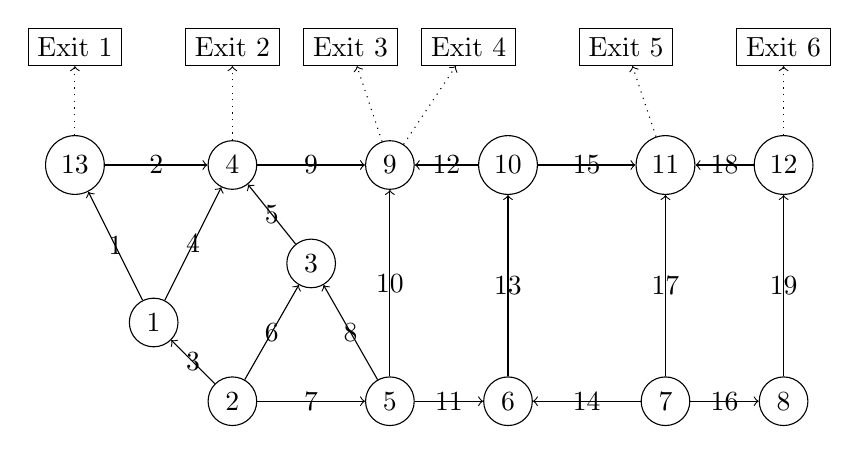
\begin{tikzpicture}

\node[draw, rectangle] (exit-1) at (0,4.5) {Exit 1};
\node[draw, rectangle] (exit-2) at (2.0,4.5) {Exit 2};
\node[draw, rectangle] (exit-3) at (3.5,4.5) {Exit 3};
\node[draw, rectangle] (exit-4) at (5.0,4.5) {Exit 4};
\node[draw, rectangle] (exit-5) at (7.0,4.5) {Exit 5};
\node[draw, rectangle] (exit-6) at (9.0,4.5) {Exit 6};

\node[draw, circle] (1) at (1.0,1.0) {$1$};
\node[draw, circle] (2) at (2.0,0.0) {$2$};
\node[draw, circle] (3) at (3.0,1.75) {$3$};
\node[draw, circle] (4) at (2.0,3.0) {$4$};
\node[draw, circle] (5) at (4.0,0.0) {$5$};
\node[draw, circle] (6) at (5.5,0.0) {$6$};
\node[draw, circle] (7) at (7.5,0.0) {$7$};
\node[draw, circle] (8) at (9.0,0.0) {$8$};
\node[draw, circle] (9) at (4.0,3.0) {$9$};
\node[draw, circle] (10) at (5.5,3.0) {$10$};
\node[draw, circle] (11) at (7.5,3.0) {$11$};
\node[draw, circle] (12) at (9.0,3.0) {$12$};
\node[draw, circle] (13) at (0,3.0) {$13$};

\draw[->] (1) to node {$1$} (13);
\draw[->] (13) to node {$2$} (4);
\draw[->] (2) to node {$3$} (1);
\draw[->] (1) to node {$4$} (4);
\draw[->] (3) to node {$5$} (4);
\draw[->] (2) to node {$6$} (3);
\draw[->] (2) to node {$7$} (5);
\draw[->] (5) to node {$8$} (3);
\draw[->] (4) to node {$9$} (9);
\draw[->] (5) to node {$10$} (9);
\draw[->] (5) to node {$11$} (6);
\draw[->] (10) to node {$12$} (9);
\draw[->] (6) to node {$13$} (10);
\draw[->] (7) to node {$14$} (6);
\draw[->] (10) to node {$15$} (11);
\draw[->] (7) to node {$16$} (8);
\draw[->] (7) to node {$17$} (11);
\draw[->] (12) to node {$18$} (11);
\draw[->] (8) to node {$19$} (12);


\draw[->, dotted] (13) to (exit-1);
\draw[->, dotted] (4) to (exit-2);
\draw[->, dotted] (9) to (exit-3);
\draw[->, dotted] (9) to (exit-4);
\draw[->, dotted] (11) to (exit-5);
\draw[->, dotted] (12) to (exit-6);


\end{tikzpicture}
\end{document}
